\chapter{Results, Snapshots and Discussions}

\section{Section 1}
To login we should enter the Account No. and Pin if the account already exits and then click
the login button or else If we want to create a new account we can directly click on New
Account button. After we click on the Login button it directs to loading page to load the
information about the customer. After login the details of the customer will be displayed. We
can also edit and save some fields. we can deposit the amount the amount which is deposited
will be updated in the balance. we can transfer the amount from one account to another we
can withdraw the amount the amount which is withdraw will be updated in the balance. It
shows the list of the customer. It shows the transaction details. It shows the balance details of
the customer. The customer can change their old pin to new pin and after changing the pin it
will be updated.\\[0.2in]
\begin{figure}[H]
\centering
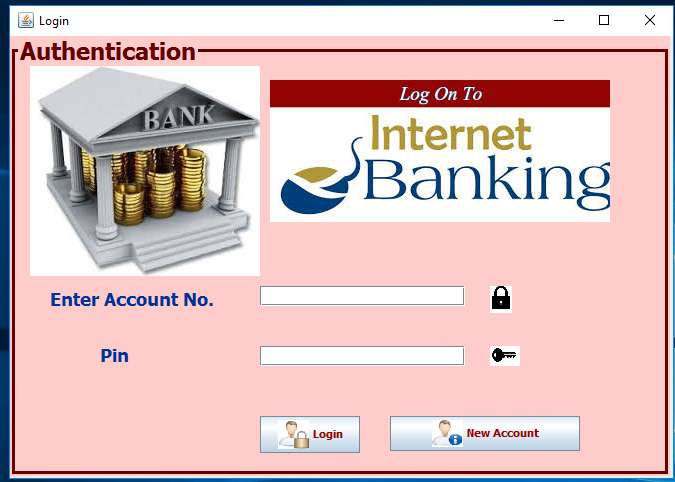
\includegraphics[scale=.5]{./loginPage.png}
\caption{Login Page}
\label{fig:Login Page}
\end{figure}
\begin{figure}[H]
\centering
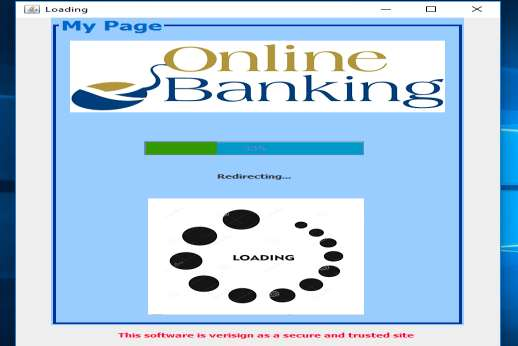
\includegraphics[scale=.5]{./loadingPage.png}]
\caption{Loading Page}
\label{fig:Loading Page}
\end{figure}
\begin{figure}[H]
\centering
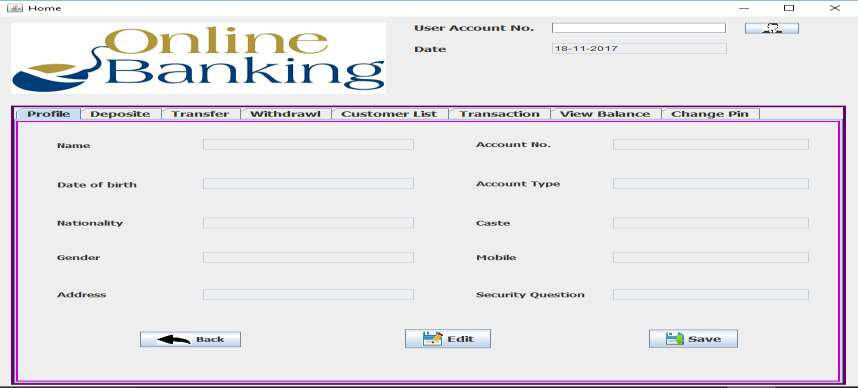
\includegraphics[scale=.5]{./profilePage.png}
\caption{Profile Page}
\label{fig:Profile Page}
\end{figure}
